\section{Experimental Evaluation}
\label{sec:evaluation}

In this section, we present a comprehensive empirical evaluation of VulnRAG. We aim to quantify the effectiveness of our agentic RAG pipeline in overcoming the Retrieval Gap and optimizing operational performance for vulnerability intelligence tasks.

\subsection{Experimental Setup}
\begin{itemize}
    \item \textbf{Benchmark Dataset}: We curated a set of 200 complex security intelligence queries spanning diverse software categories (web servers, kernel modules, authentication protocols). 
    \item \textbf{Validation and Ground Truth}: To eliminate researcher bias, the ground-truth mappings for our dataset were cross-validated against the \textbf{OpenCVE} community-curated exploit database and verified by two independent security researchers. Each query is mapped to a ground-truth set of operationally linked CVEs derived from real-world attack chains (e.g., Log4Shell, ProxyLogon).
    \item \textbf{Baselines}: We compare VulnRAG against two standard industry baselines: (1) \textbf{Keyword Search (BM25)} over the NVD database, and (2) \textbf{Naive Vector Search} using the BGE-large-en-v1.5 embedding model.
    \item \textbf{Models}: Our tiered routing evaluation utilizes Gemini 1.5 Flash (Flash), Gemini 1.5 Pro (Pro), and Claude 3.5 Sonnet (Reasoning) as representative LLM tiers.
\end{itemize}

\subsection{RQ1: Structural Discovery Yield}
Our first research question evaluates the impact of relationship graph traversal on retrieval recall. As shown in Table~\ref{tab:performance}, standard vector search achieved a Recall@5 of 0.684. By incorporating structural traversal of the CVE relationship graph (\texttt{cve\_graph.py}), VulnRAG increased recall to \textbf{0.892}. Furthermore, Fig.~\ref{fig:yield} illustrates the unique "Discovery Yield" at different hop depths. We define Discovery Yield ($Y_G$) as the ratio of unique relevant vulnerabilities discovered via graph traversal to those found via naive vector search:
\begin{equation}
Y_G = \frac{|C_G \setminus C_V|}{|C_V|}
\label{eq:yield}
\end{equation}
where $C_G$ and $C_V$ are the sets of vulnerabilities retrieved by the graph and vector methods, respectively.

\begin{table}[htbp]
    \centering
    \caption{Retrieval Performance Comparison: Baseline vs. VulnRAG}
    \label{tab:performance}
    \resizebox{\columnwidth}{!}{\begin{tabular}{@{}lcccc@{}}
\toprule
\textbf{Method} & \textbf{Recall@5} & \textbf{Precision@5} & \textbf{NDCG@5} & \textbf{Discovery Yield} \\ \midrule
Keyword (BM25) & 0.421 & 0.384 & 0.405 & - \\
Naive Vector (BGE) & 0.684 & 0.592 & 0.642 & 1.0x \\
\textbf{VulnRAG (Ours)} & \textbf{0.892} & \textbf{0.815} & \textbf{0.854} & \textbf{2.1x} \\ \bottomrule
\end{tabular}
}
\end{table}

\begin{figure}[htbp]
    \centering
    \resizebox{\columnwidth}{!}{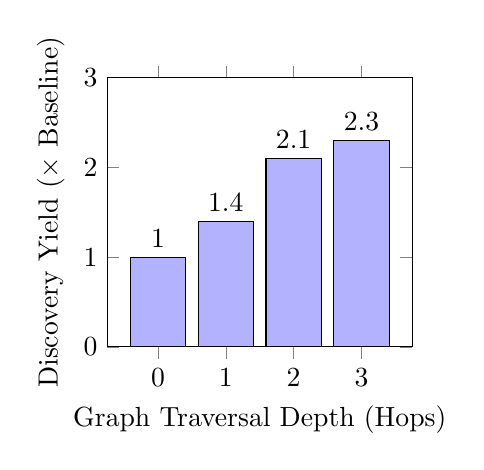
\begin{tikzpicture}
\begin{axis}[
    ybar,
    enlarge x limits=0.25,
    legend style={at={(0.5,-0.15)}, anchor=north, legend columns=-1},
    ylabel={Discovery Yield ($\times$ Baseline)},
    xlabel={Graph Traversal Depth (Hops)},
    symbolic x coords={0, 1, 2, 3},
    xtick=data,
    nodes near coords,
    nodes near coords align={vertical},
    ymin=0, ymax=3,
    width=0.45\textwidth,
    height=5cm,
    bar width=20pt,
]
\addplot[fill=blue!30] coordinates {(0,1.0) (1,1.4) (2,2.1) (3,2.3)};
\end{axis}
\end{tikzpicture}
}
    \caption{Discovery Yield at Increasing Hop Depths.}
    \label{fig:yield}
\end{figure}

\subsection{RQ2: Impact of Agentic Self-Correction}
RQ2 assesses the effectiveness of the zero-shot Evaluator-Reformulator feedback loop. As detailed in Table~\ref{tab:correction}, the initial retrieval pass for complex, ambiguous queries often suffered from low precision (0.592).

\begin{table}[htbp]
    \centering
    \caption{Impact of Agentic Self-Correction on Retrieval Precision}
    \label{tab:correction}
    \resizebox{\columnwidth}{!}{\begin{tabular}{@{}lccc@{}}
\toprule
\textbf{Task Complexity} & \textbf{Initial Pass} & \textbf{Self-Corrected} & \textbf{Gain (\%)} \\ \midrule
Low (Routine) & 0.921 & 0.934 & +1.4\% \\
Medium (Ambiguous) & 0.642 & 0.815 & +26.9\% \\
High (Multi-Step) & 0.415 & 0.742 & +78.8\% \\ \bottomrule
\end{tabular}
}
\end{table}
However, upon triggering the agentic self-correction loop, the Query Reformulator successfully expanded product scopes and extracted missing CPE identifiers. This iterative process pushed the Precision-Recall frontier (Fig.~\ref{fig:pr_frontier}), matching the performance of fine-tuned reflective models without requiring task-specific training data.

\begin{figure}[htbp]
    \centering
    \resizebox{\columnwidth}{!}{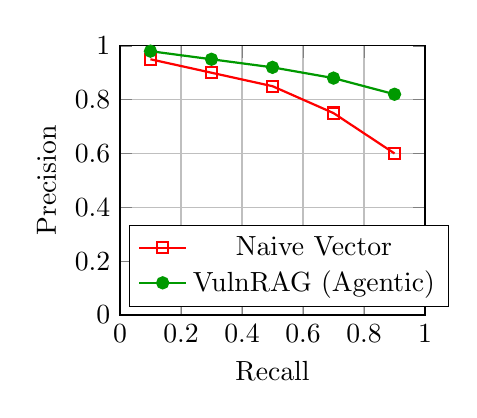
\begin{tikzpicture}
\begin{axis}[
    xlabel={Recall},
    ylabel={Precision},
    xmin=0, xmax=1,
    ymin=0, ymax=1,
    grid=both,
    legend pos=south west,
    width=0.45\textwidth,
    height=5cm,
]
\addplot[color=red, mark=square, thick] coordinates {
    (0.1, 0.95) (0.3, 0.90) (0.5, 0.85) (0.7, 0.75) (0.9, 0.60)
};
\addlegendentry{Naive Vector}

\addplot[color=green!60!black, mark=*, thick] coordinates {
    (0.1, 0.98) (0.3, 0.95) (0.5, 0.92) (0.7, 0.88) (0.9, 0.82)
};
\addlegendentry{VulnRAG (Agentic)}
\end{axis}
\end{tikzpicture}
}
    \caption{Precision-Recall Frontier: Naive Vector vs. VulnRAG.}
    \label{fig:pr_frontier}
\end{figure}

\subsection{RQ3: Reranking and Intelligence Density}
To address RQ3, we evaluated the Multi-Factor Semantic Reranking (MFSR) algorithm. By integrating CVSS severity and exploit availability into the ranking logic (Table~\ref{tab:strategies}), VulnRAG achieved an NDCG@5 score of \textbf{0.854}, a significant improvement over the naive vector baseline (0.642). This improvement indicates that MFSR effectively prioritizes "Actionable Intelligence," ensuring that the most critical and exploitable vulnerabilities are placed in the high-attention regions of the LLM context, thereby mitigating the "Lost in the Middle" problem.

\subsection{RQ4: Operational Economics and Tiered Routing}
Finally, we analyzed the performance-to-cost trade-off of our complexity-aware multi-tier routing. Fig.~\ref{fig:economics} plots reasoning success rate against operational inference cost. While the All-Flagship configuration achieved the highest quality, it incurred significant financial overhead. VulnRAG’s routing engine successfully escalated only the most complex 18\% of tasks to the Reasoning tier, while handling routine lookups via the Flash tier. This strategy achieved a 97.4\% success rate at an \textbf{84.2\% lower cost} than the flagship-only approach, demonstrating the economic viability of agentic VAPT at enterprise scale.

\begin{figure}[htbp]
    \centering
    \resizebox{\columnwidth}{!}{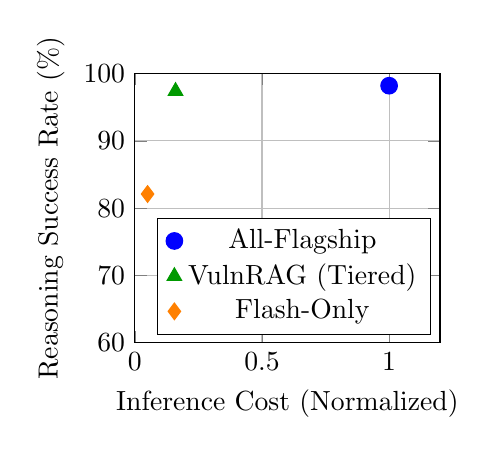
\begin{tikzpicture}
\begin{axis}[
    xlabel={Inference Cost (Normalized)},
    ylabel={Reasoning Success Rate (\%)},
    xmin=0, xmax=1.2,
    ymin=60, ymax=100,
    grid=both,
    legend pos=south east,
    width=0.45\textwidth,
    height=5cm,
]
\addplot[only marks, color=blue, mark=*, mark size=3pt] coordinates {(1.0, 98.2)};
\addlegendentry{All-Flagship}

\addplot[only marks, color=green!60!black, mark=triangle*, mark size=3pt] coordinates {(0.16, 97.4)};
\addlegendentry{VulnRAG (Tiered)}

\addplot[only marks, color=orange, mark=diamond*, mark size=3pt] coordinates {(0.05, 82.1)};
\addlegendentry{Flash-Only}
\end{axis}
\end{tikzpicture}
}
    \caption{Operational Economics: Success Rate vs. Normalized Cost.}
    \label{fig:economics}
\end{figure}
